\chapter{Angular: L'applicazione youCook}
\begin{figure}[H]
    \centering
 
\includegraphics[scale=0.2]{resources/youCook_logo.jpg}
   \caption{logo dell'applicazione}
\end{figure}
\newpage
\section{YouCook: requisiti}
Al fine di mostrare le potenzialità della libreria segue il progetto di una applicazione per la gestione e condivisione delle ricette di cucina.
L' applicazione vuole soppiantare il classico "Libro mastro delle ricette" offrendo la possibilità di monitorare, aggiornare e gestire il proprio repertorio di ricette.
I requisiti della applicazione sono i seguenti:
\begin{itemize}
    \item L'utente deve poter gestire le proprie ricette, modificarle, creare e eliminarti
    \item L'utente deve poter effetuare ricerche in base agli ingredienti principali delle ricette
    \item L' utente deve poter creare gruppi famiglia all'interno dei quali selezionare fra le ricette il "Pasto del giorno" ovvero la ricetta che si intende realizzare per il pasto selezionato "pranzo, cena"
    \item all'interno del gruppo famiglia l'utente deve poter amministrare i membri 
    
\end{itemize}
L'applicazione ha inoltre come obbiettivo quello di mettere in luce le potenzialità della strategia di change detection onPush.
\newpage
\subsection{Tabella dei requisiti}
\FloatBarrier
\begin{longtable}{|p{2.5cm}|p{9cm}|p{2.5cm}|}
\hline

\endfirsthead
\multicolumn{3}{c}%
{\tablename\ \thetable\ -- \textit{Continued from previous page}} \\
\hline
 \rowcolor{white}\textbf{ID} & \textbf{REQUISITO} & \textbf{TIPO} \\
\hline
\endhead
\hline \multicolumn{3}{r}{\textit{Continued on next page}} \\
\endfoot
\hline
\endlastfoot

\rowcolor{white}\textbf{ID} & \textbf{REQUISITO} & \textbf{TIPO} \\
         \hline
         R1F &L'applicazione deve fornire una funzionalità di registrazione agli utenti & Funzionale\\
         
         \hline
         R2F &L'applicazione deve dare la possibilità di aggiungere modificare e eliminare le proprie ricette&Funzionale \\
         
         \hline
         R3F &L'acquirente deve poter effettuare ricerche in base agli ingredienti & Funzionale \\
         
         \hline
         R4F &L'applicazione deve poter permettere all'utente di creare gruppi famiglia&Funzionale \\
         
         \hline
         R5F &L'applicazione deve poter permettere all'utente di amministrare i gruppi famiglia, rimuovendo o aggiungendo mebri al gruppo &Funzionale \\
         
         \hline
         R6F & L'applicazione deve consentire all'utente di selezionare il "pasto del giorno"&Funzionale \\

\end{longtable}
\FloatBarrier
\newpage
\begin{figure}[H]
    \centering
 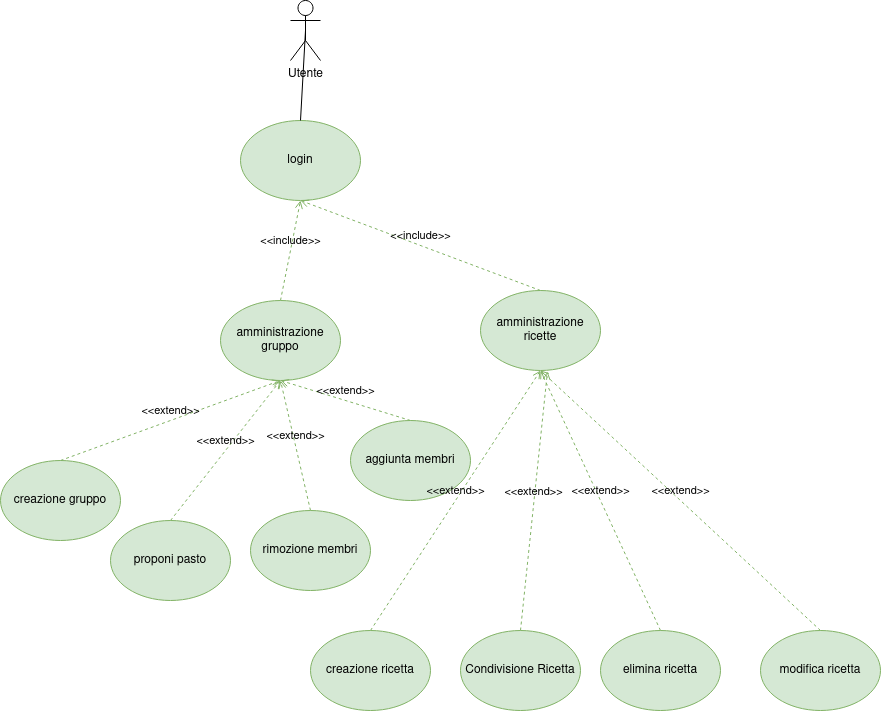
\includegraphics[scale=0.5]{resources/diagramma_casi_uso.drawio.png}
   \caption{Diagramma casi d'uso della applicazione}
\end{figure}
Il diagramma mette in luce le principali funzionalità fornite all'utente che, dopo la procedura di login, può visualizzare il proprio elenco di ricette e interagire con lo stesso  oppure visionare i membri del gruppo famiglia a lui associato.